All results calculated with $95\%$ confidence-interval and margin of error for each of them less than $2.5\%$. We have used tool to calculate $95\%$ confidence interval from
\href{https://www.mathsisfun.com/data/confidence-interval-calculator.html}{$Confidence\_Interval\_Calculator$}
\subsection{Experiment I}
\begin{figure}[ht]
   \centering
   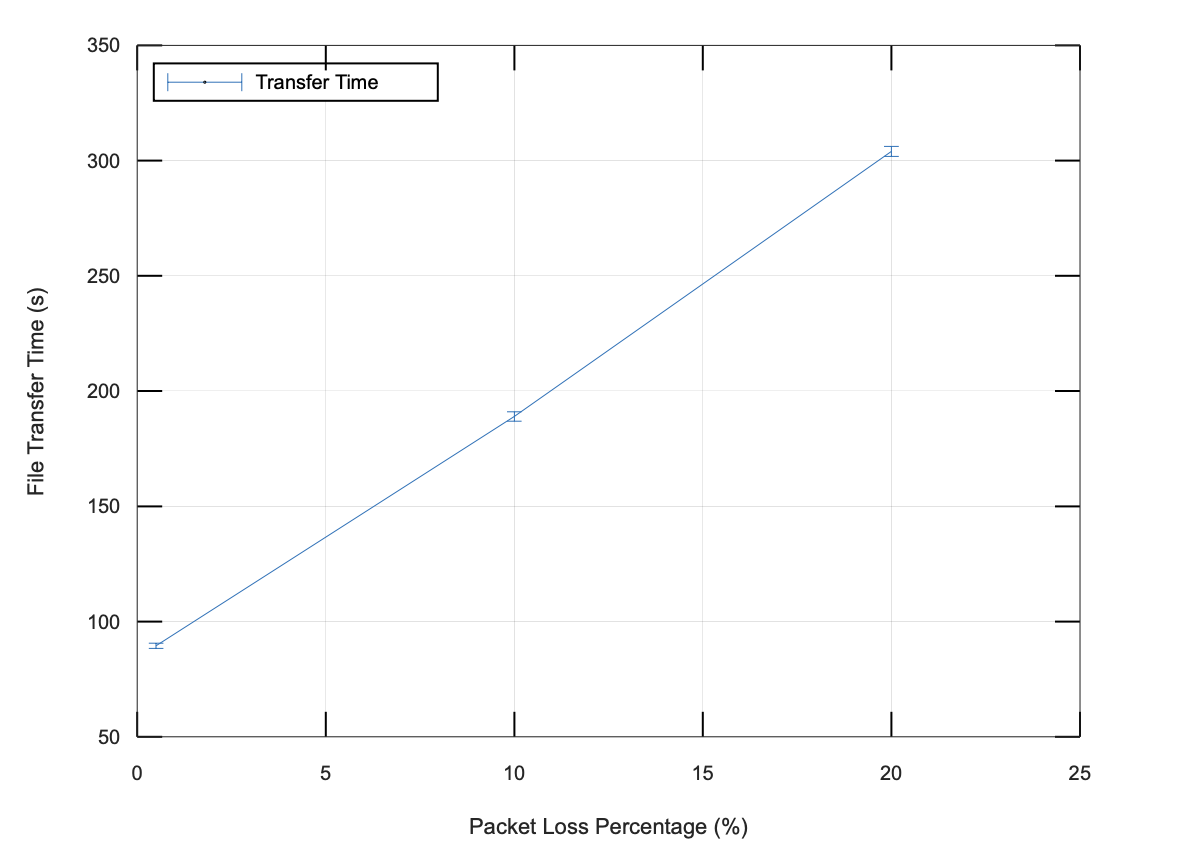
\includegraphics[scale=.45]{images/exp1.png}
    \caption{File Transfer Time(s) vs Packet Loss Percentage(\%)}
    \label{fig:topology}
\end{figure}
The confidence intervals are :

$89.5 \pm 1.12$

$189 \pm 2.04$

$304 \pm 2.16$\\
Our protocol is reliable, so when packet loss occurs, re-transmission starts with Go-Back-N, then sent lost packets again. As we can see from the Figure 1, when packet loss percentage increased, file transfer time also increased because there were more re-transmitted packets. As a result, we have observed that packet loss percentage and file transfer time is directly proportional to each other.
\newpage
\subsection{Experiment II}
\begin{figure}[ht]
   \centering
   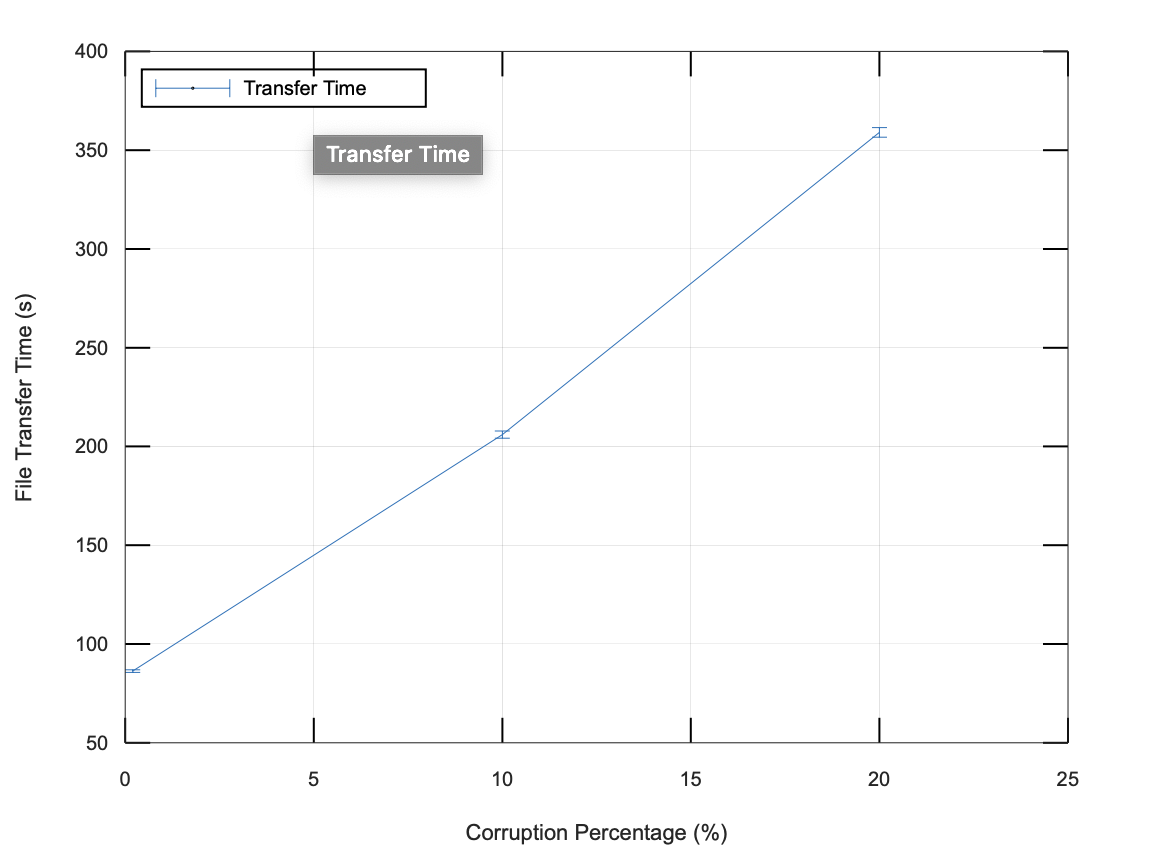
\includegraphics[scale=.45]{images/exp2.png}
    \caption{File Transfer Time(s) vs Corruption Percentage(\%)}
    \label{fig:topology}
\end{figure}
The confidence intervals are :

$86.3 \pm 0.627$

$206 \pm 1.8$

$359 \pm 2.42$\\
We used mechanisms use to provide reliability, one of them is checksum. When checksum value in the header and re-calculated checksum value doesn't match, it means that there is corruption in packets. When corrupted data received at destination, re-transmission starts with Go-Back-N, then sent corrupted packets again. As we can see from the Figure 2, when corruption percentage increased, file transfer time also increased because there were more re-transmitted packets. As a result, we have observed that corruption percentage and file transfer time is proportional to each other.
\subsection{Experiment III}
\begin{figure}[ht]
   \centering
   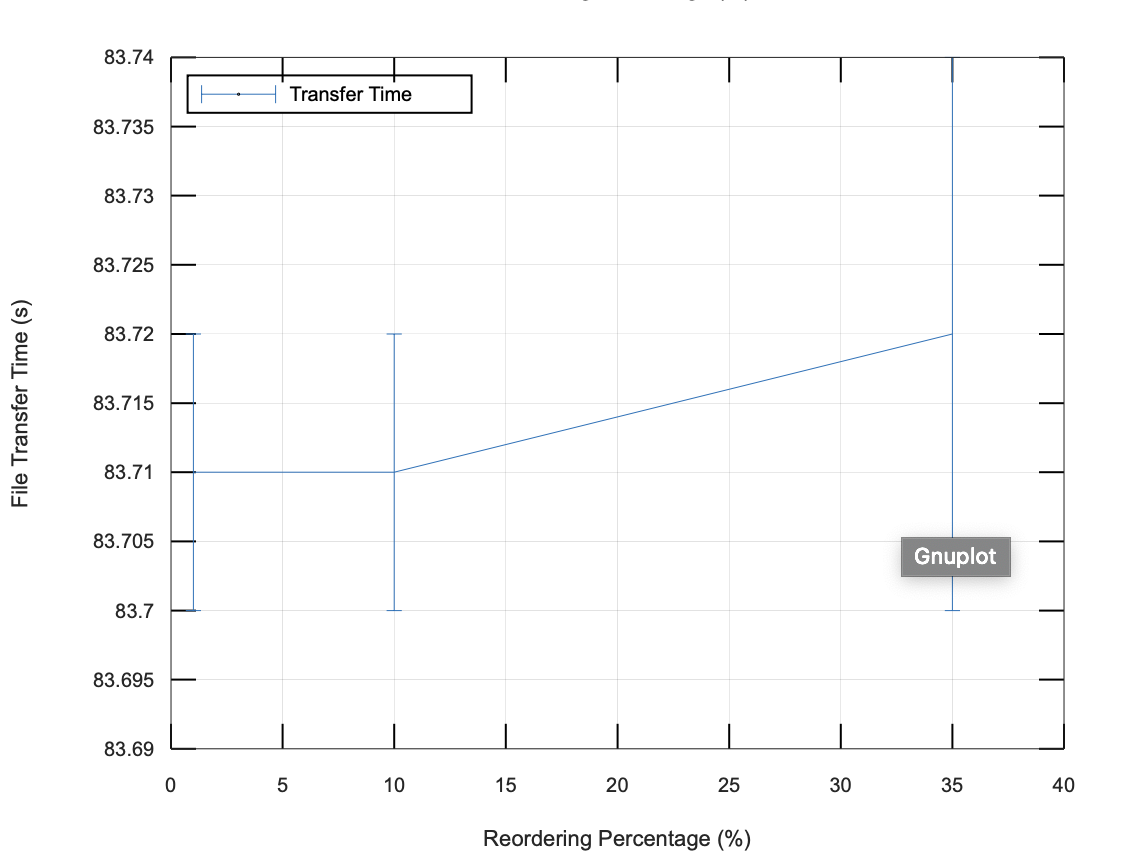
\includegraphics[scale=.45]{images/exp3.png}
    \caption{File Transfer Time(s) vs Reordering Percentage(\%)}
    \label{fig:topology}
\end{figure}
The confidence intervals are :

$ 83.7 \pm 0.01$

$83.7 \pm 0.01$

$83.71 \pm 0.02$\\
We implemented Go-Back-N mechanism to our protocol, but not same. 
In the results, we have observed that there are little changes in file transfer time for different re-ordering percentages. That might be caused because of we are starting threads separately in broker node, means either $1$ thread starts, or the other one. In theory, when re-ordering percentages changes, file transfer time should also be changes in Go-Back-N, but in our cases there is no slightly change in graph. When we add re-ordering percentage, since threads doesn't affected with them, there were no slightly changes in graph.